\section{Etapa 5 – Resultados del modelado predictivo y evaluativo}
\label{sec:resultados-etapa5}

Los resultados de esta sección corresponden a la re-estimación final de la Etapa~5 (\texttt{Etapa5\_09\_reestimacion\_v3.Rmd}), que sustituye a la re-estimación de cierre de la versión anterior del documento. Respecto de los informes preliminares, la especificación incorpora cinco decisiones: (i)~todas las predictoras observadas en la semana~$s$ entran rezagadas una semana; (ii)~se excluyen las dos variables de activos construidas con fechas posteriores al periodo pronosticado; (iii)~los rezagos propio y espacial de la respuesta entran en la escala $\log(1+y)$ de la ecuación~\eqref{eq:especificacion_panel}; (iv)~todos los modelos se evalúan sobre una muestra común frente a dos pronósticos de referencia; y (v)~la inferencia sobre las diferencias de error toma la semana como unidad e incluye intervalos por remuestreo de bloques (Sección~\ref{sec:evaluacion_desempeno}). Las variables sísmicas son las reconstruidas tras corregir los dos errores de integración descritos en la Sección~\ref{sec:sismicidad_sgc}.

\subsection{Dependencia espacial}
\label{sec:resultados_moran}

El diagnóstico de dependencia espacial confirmó autocorrelación positiva y significativa en el promedio por cuadrante tanto de SAIDI (índice de Moran $I=0{.}154$; $p<0{.}001$) como de SAIFI ($I=0{.}179$; $p<0{.}001$), y en el corte transversal ponderado ($I=0{.}146$ y $I=0{.}240$, respectivamente; $p<0{.}001$). La magnitud es moderada: la vecindad territorial explica una parte identificable pero no dominante de la variación, lo que justifica incorporar rezagos espaciales y estimar SAR y SEM, sin anticipar que estos dominen a los modelos no espaciales.

\subsection{Muestra de evaluación}
\label{sec:resultados_muestra}

La Tabla~\ref{tab:flujo_muestra} presenta el flujo de inclusión de la muestra de magnitud. De las $13\,351$ semanas con falla de $D_{\mathrm{mod}}$, $11\,136$ pertenecen al entrenamiento y $2\,215$ al periodo de prueba, comprendido entre el 15 de septiembre y el 29 de diciembre de 2025. El entrenamiento pierde $184$ filas por rezagos no definidos en las primeras semanas de cada serie, y la prueba no pierde ninguna. La muestra común de evaluación excluye solo tres observaciones de un cuadrante que no registró fallas en el entrenamiento y para el que, por tanto, ni el efecto fijo ni la media del cuadrante están definidos; todas las métricas de magnitud que siguen se calculan sobre esas mismas $2\,212$ llaves cuadrante--semana. El clasificador de ocurrencia, que solo exige completitud en las variables que utiliza, se evalúa sobre las $5\,504$ semanas del periodo de prueba, con y sin falla.

\begin{table}[!htbp]
\centering
\small
\caption{Flujo de inclusión de la muestra de magnitud (semanas con falla)}
\label{tab:flujo_muestra}
\begin{adjustbox}{max width=\linewidth}
\begin{tabular}{p{0.46\textwidth} r r r r}
\toprule
& \multicolumn{2}{c}{\textbf{SAIDI}} & \multicolumn{2}{c}{\textbf{SAIFI}} \\
\cmidrule(lr){2-3}\cmidrule(lr){4-5}
\textbf{Paso} & \textbf{Filas} & \textbf{Cuadrantes} & \textbf{Filas} & \textbf{Cuadrantes} \\
\midrule
Filas cuadrante-semana del panel & 36\,120 & 344 & 36\,120 & 344 \\
Semanas con falla & 13\,351 & 324 & 13\,351 & 324 \\
Entrenamiento con falla (hasta el corte) & 11\,136 & 323 & 11\,136 & 323 \\
Entrenamiento con predictoras completas & 10\,952 & 323 & 10\,952 & 323 \\
Prueba con falla (después del corte) & 2\,215 & 294 & 2\,215 & 294 \\
Prueba con predictoras completas & 2\,215 & 294 & 2\,215 & 294 \\
Muestra común (cuadrante visto en entrenamiento) & 2\,212 & 293 & 2\,212 & 293 \\
\bottomrule
\end{tabular}

\end{adjustbox}
\end{table}

\subsection{Pronóstico semanal frente a pronósticos de referencia}
\label{sec:resultados_pronostico}

Las Tablas~\ref{tab:desempeno_saidi} y~\ref{tab:desempeno_saifi} presentan el desempeño de los modelos de panel y de dos pronósticos de referencia: la \textit{persistencia}, que pronostica para cada cuadrante el valor de su semana anterior, y la \textit{media del cuadrante}, que pronostica su promedio histórico en el entrenamiento. El modelo de efectos fijos de cuadrante y semana no es evaluable fuera de muestra, porque las semanas de prueba no tienen efecto fijo estimado (Sección~\ref{sec:validacion_modelo}), y no se incluye en las tablas.

\begin{table}[!htbp]
\centering
\small
\caption{Desempeño en el conjunto de prueba para SAIDI (escala $\log(1+y)$; muestra común, $N=2\,212$)}
\label{tab:desempeno_saidi}
\begin{adjustbox}{max width=\linewidth}
\begin{tabular}{l r r r r r r}
\toprule
\textbf{Modelo} & \textbf{RMSE} & \textbf{MAE} & \textbf{$r^2$} & \makecell[c]{\textbf{$R^2$}\\\textbf{predictivo}} & \makecell[c]{\textbf{MAE rel.}\\\textbf{persistencia}} & \textbf{MASE} \\
\midrule
Persistencia ($t-1$) & 0.1278 & 0.0378 & 0.120 & -0.321 & 1.000 & 0.995 \\
Media del cuadrante & 0.1030 & 0.0361 & 0.207 & 0.142 & 0.956 & 0.952 \\
\emph{Pooled} OLS & 0.1012 & 0.0376 & 0.209 & 0.173 & 0.997 & 0.992 \\
FE cuadrante & \textbf{0.1011} & 0.0366 & 0.225 & 0.174 & 0.969 & 0.964 \\
Random Forest ajustado & 0.1108 & 0.0447 & 0.200 & 0.008 & 1.183 & 1.177 \\
\bottomrule
\end{tabular}

\end{adjustbox}
\end{table}

\begin{table}[!htbp]
\centering
\small
\caption{Desempeño en el conjunto de prueba para SAIFI (escala $\log(1+y)$; muestra común, $N=2\,212$)}
\label{tab:desempeno_saifi}
\begin{adjustbox}{max width=\linewidth}
\begin{tabular}{l r r r r r r}
\toprule
\textbf{Modelo} & \textbf{RMSE} & \textbf{MAE} & \textbf{$r^2$} & \makecell[c]{\textbf{$R^2$}\\\textbf{predictivo}} & \makecell[c]{\textbf{MAE rel.}\\\textbf{persistencia}} & \textbf{MASE} \\
\midrule
Persistencia ($t-1$) & 0.00324 & 0.00081 & 0.085 & -0.413 & 1.000 & 0.926 \\
Media del cuadrante & \textbf{0.00238} & 0.00071 & 0.261 & 0.240 & 0.881 & 0.816 \\
\emph{Pooled} OLS & 0.00243 & 0.00080 & 0.221 & 0.208 & 0.986 & 0.913 \\
FE cuadrante & 0.00239 & 0.00073 & 0.257 & 0.233 & 0.907 & 0.840 \\
Random Forest ajustado & 0.00253 & 0.00092 & 0.225 & 0.136 & 1.143 & 1.058 \\
\bottomrule
\end{tabular}

\end{adjustbox}

\vspace{2pt}
\noindent\footnotesize\textit{Nota:} $r^2$, cuadrado de la correlación de Pearson; $R^2$ predictivo y MASE según las ecuaciones~\eqref{eq:metricas} y~\eqref{eq:mase}; MAE relativo, cociente con el MAE de la persistencia en las mismas observaciones de prueba.
\end{table}

La Tabla~\ref{tab:diebold_mariano} contrasta las diferencias con la prueba de Diebold--Mariano semanal de la ecuación~\eqref{eq:dm_semanal} y reporta la mejora porcentual del RMSE con su intervalo por remuestreo de bloques. Tres resultados se desprenden de ella. Primero, los modelos lineales superan con claridad a la persistencia: FE de cuadrante reduce el RMSE en un $20{.}9$~\% en SAIDI y en un $26{.}3$~\% en SAIFI, con intervalos alejados de cero y $p\leq0{.}005$. Segundo, no se demostró una mejora sobre la media histórica del cuadrante. En SAIDI, FE de cuadrante reduce el RMSE en un $1{.}8$~\%, pero el intervalo incluye el cero ($-0{.}2$ a $3{.}1$~\%) y la prueba no es significativa al $5$~\% ($p=0{.}063$); en SAIFI, la media del cuadrante es incluso ligeramente mejor ($0{.}5$~\%; $p=0{.}30$). Con dieciséis semanas de prueba, esta ausencia de significancia no equivale a que ambos pronósticos sean iguales: indica que, con estos datos y este diseño, la ganancia de FE sobre la media, si existe, es pequeña. Tercero, Random Forest es inferior a FE de cuadrante en ambos indicadores ($9{.}6$~\% y $6{.}1$~\% más RMSE; $p=0{.}003$), y su MAE supera incluso al de la persistencia.

\begin{table}[!htbp]
\centering
\small
\caption{Diebold--Mariano semanal y mejora del RMSE con intervalo por remuestreo de bloques de semanas ($T=16$)}
\label{tab:diebold_mariano}
\begin{adjustbox}{max width=\linewidth}
\begin{tabular}{l l r r r c}
\toprule
\textbf{Indicador} & \textbf{Comparación} & \textbf{DM} & \textbf{valor $p$} & \makecell[c]{\textbf{Mejora}\\\textbf{RMSE (\%)}} & \makecell[c]{\textbf{IC 95~\%}\\\textbf{(bloques)}} \\
\midrule
SAIDI & RF ajustado vs.\ FE cuadrante & $3{.}48$ & $0{.}003$ & $-9{.}6$ & $[-22{.}0;\ -4{.}4]$ \\
 & FE cuadrante vs.\ persistencia ($t-1$) & $-3{.}33$ & $0{.}005$ & $20{.}9$ & $[15{.}6;\ 28{.}5]$ \\
 & FE cuadrante vs.\ media del cuadrante & $-2{.}01$ & $0{.}063$ & $1{.}8$ & $[-0{.}2;\ 3{.}1]$ \\
\addlinespace
SAIFI & RF ajustado vs.\ FE cuadrante & $3{.}51$ & $0{.}003$ & $-6{.}1$ & $[-12{.}4;\ -2{.}6]$ \\
 & FE cuadrante vs.\ persistencia ($t-1$) & $-3{.}87$ & $0{.}002$ & $26{.}3$ & $[20{.}5;\ 34{.}8]$ \\
 & FE cuadrante vs.\ media del cuadrante & $1{.}08$ & $0{.}296$ & $-0{.}5$ & $[-1{.}0;\ 0{.}0]$ \\
\bottomrule
\end{tabular}

\end{adjustbox}

\vspace{2pt}
\noindent\footnotesize\textit{Nota:} un estadístico negativo indica que el primer modelo tiene menor error cuadrático; la mejora es $100\,(1-\mathrm{RMSE}_A/\mathrm{RMSE}_B)$. Intervalos por remuestreo de bloques móviles de tres semanas ($2\,000$ réplicas).
\end{table}

En la escala original del indicador, con la corrección de \emph{smearing} de Duan, FE de cuadrante obtiene un RMSE de $0{.}171$ en SAIDI frente a $0{.}203$ de la media del cuadrante y un MAE de $0{.}050$ frente a $0{.}054$. En SAIFI, la media del cuadrante conserva una ligera ventaja ($0{.}00242$ frente a $0{.}00243$). El factor de corrección es pequeño ($1{.}009$ en SAIDI y prácticamente $1$ en SAIFI), porque la varianza residual en escala logarítmica es reducida.

La lectura conjunta es consistente: casi toda la capacidad predictiva semanal proviene del \textit{nivel propio de cada cuadrante}. El $R^2$ predictivo de FE de cuadrante, de $0{.}17$ en SAIDI y $0{.}23$ en SAIFI, es del mismo orden que el de la media del cuadrante ($0{.}14$ y $0{.}24$). Una vez conocido el nivel típico de afectación del cuadrante, las variables que cambian de semana a semana ---clima rezagado, NDVI y sismicidad--- aportan poca información adicional. En SAIDI, los únicos términos dinámicos con efecto son el rezago propio ($\hat\gamma=0{.}162$; $p<0{.}001$ con errores agrupados por cuadrante y con errores de Driscoll--Kraay) y, con menor solidez, el rezago de los vecinos ($\hat\phi=0{.}092$; $p=0{.}041$ agrupado y $p=0{.}053$ Driscoll--Kraay). En SAIFI ningún término dinámico es significativo, y ninguna variable climática, de vegetación o sísmica rezagada lo es en ninguno de los dos indicadores. Todos los contrastes usan errores robustos a heterocedasticidad y a correlación dentro del cuadrante. Los factores de inflación de varianza son altos para el par \texttt{prop\_estrato\_1}--\texttt{prop\_estrato\_2} ($25$ y $24$) y moderados para \texttt{n\_elementos} y \texttt{longitud\_red\_km} ($16$ y $15$); ninguna variable dinámica tiene un VIF superior a $5$, de modo que la colinealidad no explica la ausencia de significancia de las variables semanales.

El bajo desempeño de Random Forest es coherente con lo anterior. La búsqueda de hiperparámetros (Tabla~\ref{tab:tuning_rf} y Figura~\ref{fig:tuning_rf}) seleccionó en ambos indicadores el valor mínimo de \texttt{mtry} ($2$), la configuración más regularizada de la grilla, que es el patrón esperado cuando la señal es débil y el modelo tiende a ajustar ruido.

\begin{table}[!htbp]
\centering
\small
\caption{Ajuste de hiperparámetros del Random Forest: mejores configuraciones según la validación temporal interna}
\label{tab:tuning_rf}
\begin{adjustbox}{max width=\linewidth}
\begin{tabular}{l r r r}
\toprule
\textbf{Indicador} & \textbf{\texttt{mtry}} & \textbf{Tamaño mínimo de nodo} & \textbf{RMSE validación interna} \\
\midrule
SAIDI & 2 & 10 & 0.1250 \\
 & 2 & 20 & 0.1252 \\
 & 2 & 5 & 0.1253 \\
\addlinespace
SAIFI & 2 & 20 & 0.00247 \\
 & 2 & 50 & 0.00249 \\
 & 4 & 50 & 0.00249 \\
\bottomrule
\end{tabular}

\end{adjustbox}

\vspace{2pt}
\noindent\footnotesize\textit{Nota:} grilla de $6\times4$ combinaciones ($\texttt{mtry}\in\{2,4,6,9,12,16\}$; tamaño mínimo de nodo $\in\{5,10,20,50\}$), estimadas con \texttt{ranger} ($500$ árboles) sobre el $85$~\% inicial de las semanas de entrenamiento y evaluadas en las restantes. El conjunto de prueba no interviene en el ajuste.
\end{table}

\begin{figure}[!htbp]
    \centering
    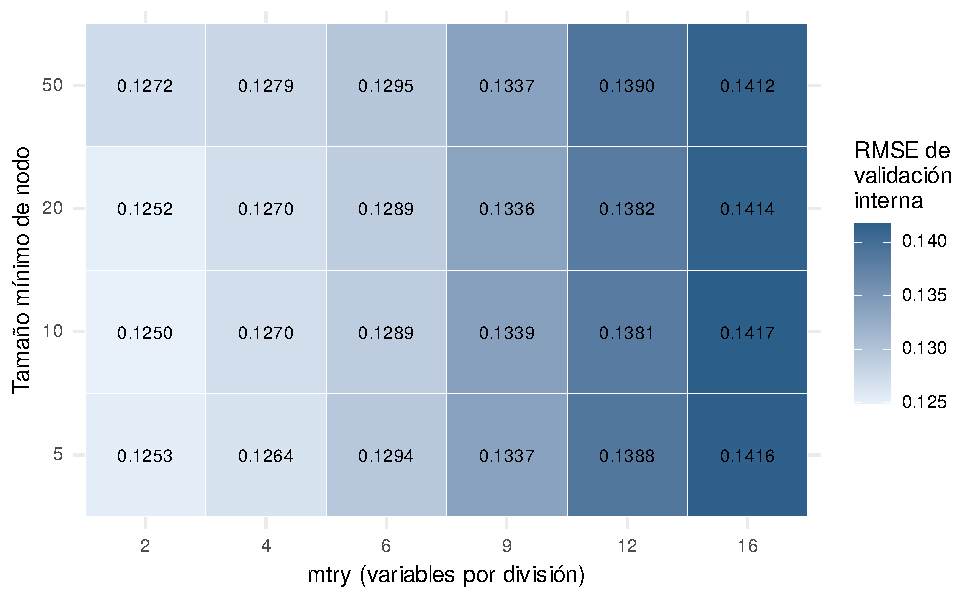
\includegraphics[width=0.80\textwidth]{img/fig_tuning_rf_SAIDI.pdf}
    \caption{RMSE de validación interna del Random Forest de SAIDI según \texttt{mtry} y tamaño mínimo de nodo.}
    \label{fig:tuning_rf}
\end{figure}

La validación de origen móvil (Tabla~\ref{tab:origen_movil}) repite la estimación en cuatro cortes, con la selección de hiperparámetros anidada en el pasado de cada uno. La persistencia es el peor pronóstico en los ocho casos. Entre los demás, ningún modelo domina: en SAIDI, Random Forest obtiene el menor error en los dos primeros cortes, la media del cuadrante en el tercero y FE de cuadrante en el cuarto; en SAIFI, Random Forest es mejor en los dos primeros y la media del cuadrante en los dos últimos. Las diferencias entre FE, \emph{Pooled} OLS, Random Forest y la media del cuadrante son pequeñas frente a la variación entre cortes, mientras que la ventaja de todos ellos sobre la persistencia es grande y sistemática. La configuración elegida para el Random Forest también varía entre cortes, lo que confirma que el ajuste de hiperparámetros no encuentra una estructura estable.

\begin{table}[!htbp]
\centering
\small
\caption{Validación de origen móvil: RMSE en las doce semanas siguientes a cada corte (escala $\log(1+y)$)}
\label{tab:origen_movil}
\begin{adjustbox}{max width=\linewidth}
\begin{tabular}{l c r r c r r r r r}
\toprule
\textbf{Ind.} & \textbf{Origen} & \makecell[c]{$n$\\entren.} & \makecell[c]{$n$\\prueba} & \makecell[c]{\texttt{mtry}/\\nodo} & \makecell[c]{Persis-\\tencia} & \makecell[c]{Media del\\cuadrante} & \makecell[c]{\emph{Pooled}\\OLS} & \makecell[c]{FE\\cuadrante} & \makecell[c]{RF\\ajustado} \\
\midrule
SAIDI & 23/12/2024 & 5\,939 & 1\,337 & 6/50 & 0.1026 & 0.0941 & 0.0898 & 0.0906 & \textbf{0.0875} \\
 & 17/03/2025 & 7\,277 & 1\,698 & 6/50 & 0.1218 & 0.1002 & 0.0958 & 0.0966 & \textbf{0.0942} \\
 & 09/06/2025 & 8\,978 & 1\,796 & 16/50 & 0.1692 & \textbf{0.1290} & 0.1325 & 0.1293 & 0.1439 \\
 & 01/09/2025 & 10\,778 & 1\,874 & 3/10 & 0.1331 & 0.1051 & 0.1039 & \textbf{0.1032} & 0.1210 \\
SAIFI & 23/12/2024 & 5\,939 & 1\,337 & 3/50 & 0.00255 & 0.00214 & 0.00216 & 0.00213 & \textbf{0.00210} \\
 & 17/03/2025 & 7\,277 & 1\,698 & 3/50 & 0.00341 & 0.00252 & 0.00256 & 0.00251 & \textbf{0.00249} \\
 & 09/06/2025 & 8\,978 & 1\,796 & 3/50 & 0.00348 & \textbf{0.00252} & 0.00268 & 0.00252 & 0.00253 \\
 & 01/09/2025 & 10\,778 & 1\,874 & 3/50 & 0.00292 & \textbf{0.00210} & 0.00221 & 0.00211 & 0.00236 \\
\bottomrule
\end{tabular}

\end{adjustbox}

\vspace{2pt}
\noindent\footnotesize\textit{Nota:} en cada corte, modelos, media del cuadrante e hiperparámetros del Random Forest se estiman solo con las semanas anteriores; en negrita, el menor RMSE de cada fila.
\end{table}

\subsection{Pronóstico de la ocurrencia de falla}
\label{sec:resultados_ocurrencia}

Los modelos anteriores pronostican la magnitud \textit{condicional} a que ocurra al menos una falla. Para completar el esquema en dos partes señalado en la Sección~\ref{sec:segmentacion_analitica}, se estimó un clasificador Random Forest de la ocurrencia de falla (\texttt{hubo\_falla}) sobre el panel completo, con las mismas predictoras \emph{ex ante} más el indicador de falla de la semana anterior. La Tabla~\ref{tab:ocurrencia} lo compara con tres referencias. En el periodo de prueba, en el que el $40{.}2$~\% de las semanas--cuadrante registró al menos una falla, el clasificador alcanza un AUC de $0{.}835$ y un AUC de precisión--exhaustividad de $0{.}773$, muy por encima de la persistencia ($0{.}721$). Sin embargo, la tasa histórica de falla de cada cuadrante en el entrenamiento, que no usa ninguna variable semanal, discrimina ligeramente mejor (AUC de $0{.}845$) y está mejor calibrada (Brier de $0{.}158$ frente a $0{.}162$); la diferencia de AUC es pequeña pero su intervalo excluye el cero ($-0{.}027$ a $-0{.}002$). El Random Forest supera, en cambio, a la regresión logística con las mismas predictoras.

\begin{table}[!htbp]
\centering
\small
\caption{Ocurrencia de falla en el periodo de prueba: discriminación, calibración y comparación con referencias ($N=5\,504$)}
\label{tab:ocurrencia}
\begin{adjustbox}{max width=\linewidth}
\begin{tabular}{l r r r r}
\toprule
\textbf{Modelo} & \textbf{AUC} & \textbf{AUC-PR} & \textbf{Brier} & \textbf{Log-loss} \\
\midrule
Random Forest & 0.835 & 0.773 & 0.1621 & 0.4886 \\
Regresión logística & 0.822 & 0.747 & 0.1712 & 0.5122 \\
Tasa histórica del cuadrante & 0.845 & 0.781 & 0.1576 & 0.4763 \\
Persistencia ($t-1$) & 0.721 & 0.651 & 0.2727 & 2.5118 \\
\midrule
\multicolumn{5}{l}{\textit{Diferencias con IC del 95~\% por remuestreo de bloques de semanas}} \\
\textbf{Comparación} & \multicolumn{2}{c}{\textbf{$\Delta$AUC}} & \multicolumn{2}{c}{\textbf{$\Delta$Brier}} \\
\midrule
Random Forest vs.\ tasa histórica del cuadrante & \multicolumn{2}{c}{$-0{.}010$ $[-0{.}027;\ -0{.}002]$} & \multicolumn{2}{c}{$0{.}0045$ $[0{.}0001;\ 0{.}0134]$} \\
Regresión logística vs.\ tasa histórica del cuadrante & \multicolumn{2}{c}{$-0{.}024$ $[-0{.}042;\ -0{.}017]$} & \multicolumn{2}{c}{$0{.}0136$ $[0{.}0095;\ 0{.}0205]$} \\
Random Forest vs.\ regresión logística & \multicolumn{2}{c}{$0{.}014$ $[0{.}006;\ 0{.}022]$} & \multicolumn{2}{c}{$-0{.}0091$ $[-0{.}0131;\ -0{.}0052]$} \\
\bottomrule
\end{tabular}

\end{adjustbox}
\end{table}

Las probabilidades del clasificador están razonablemente calibradas (Figura~\ref{fig:calibracion_ocurrencia}): en el decil de mayor probabilidad la tasa observada de falla es del $90{.}6$~\%, para una probabilidad media pronosticada del $86{.}4$~\%, y en el decil más bajo es del $2{.}2$~\%, con ligera subestimación en los deciles altos. La utilidad operativa se evaluó como lo haría una cuadrilla con capacidad fija (Tabla~\ref{tab:topk}): si cada semana se atendieran los diez cuadrantes de mayor probabilidad, el $92{.}5$~\% de ellos habría registrado efectivamente una falla y se habría cubierto el $37{.}6$~\% del SAIDI semanal; con la tasa histórica, el $97{.}5$~\% y el $36{.}5$~\%, respectivamente. Con treinta cuadrantes, las cuatro reglas capturan entre el $53$ y el $56$~\% del SAIDI semanal.

\begin{figure}[!htbp]
    \centering
    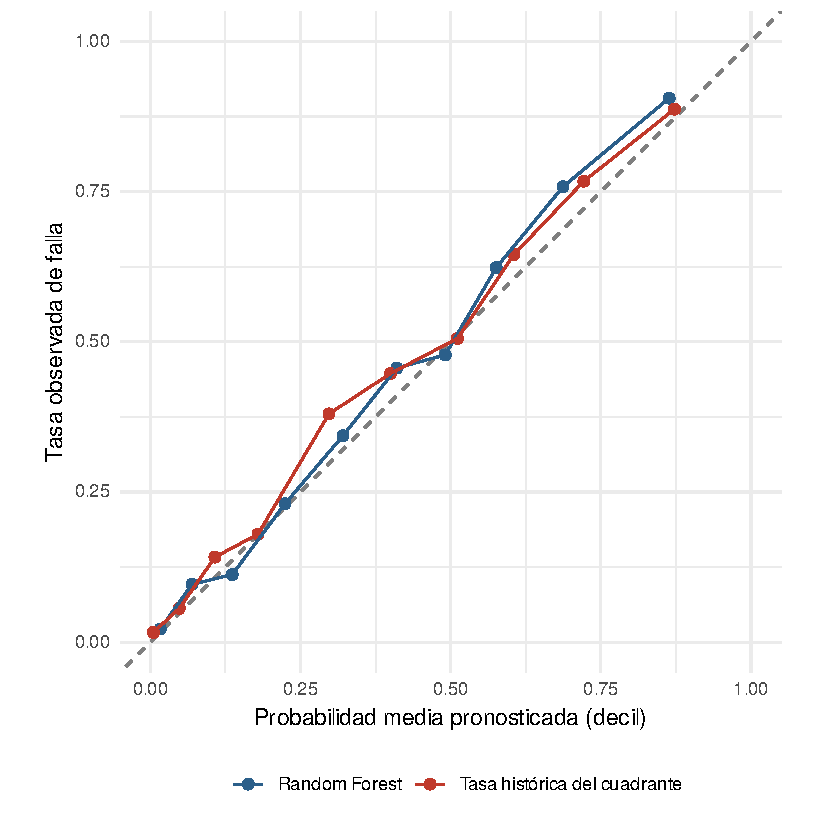
\includegraphics[width=0.58\textwidth]{img/fig_calibracion_ocurrencia.pdf}
    \caption{Confiabilidad de la probabilidad semanal de falla por decil en el periodo de prueba: Random Forest y tasa histórica del cuadrante.}
    \label{fig:calibracion_ocurrencia}
\end{figure}

\begin{table}[!htbp]
\centering
\small
\caption{Captura semanal entre los $k$ cuadrantes de mayor probabilidad de falla (promedio de las $16$ semanas de prueba)}
\label{tab:topk}
\begin{adjustbox}{max width=\linewidth}
\begin{tabular}{c l r r r}
\toprule
\textbf{$k$} & \textbf{Criterio de orden} & \makecell[c]{\textbf{Precisión}\\\textbf{(\%)}} & \makecell[c]{\textbf{SAIDI}\\\textbf{capturado (\%)}} & \makecell[c]{\textbf{SAIFI}\\\textbf{capturado (\%)}} \\
\midrule
10 & Random Forest & 92.5 & 37.6 & 37.6 \\
 & Regresión logística & 93.8 & 37.1 & 36.2 \\
 & Tasa histórica del cuadrante & 97.5 & 36.5 & 34.4 \\
 & Persistencia ($t-1$) & 96.9 & 36.5 & 34.2 \\
30 & Random Forest & 88.8 & 52.9 & 53.4 \\
 & Regresión logística & 86.0 & 55.4 & 56.1 \\
 & Tasa histórica del cuadrante & 89.4 & 55.9 & 56.9 \\
 & Persistencia ($t-1$) & 89.0 & 54.4 & 57.1 \\
\bottomrule
\end{tabular}

\end{adjustbox}
\end{table}

La ocurrencia de falla es, por tanto, pronosticable con una precisión útil, pero esa capacidad proviene casi por completo de la propensión histórica de cada cuadrante: las variables semanales no mejoran el orden que ya ofrece la tasa histórica. La probabilidad semanal sirve para ordenar los cuadrantes según su riesgo de falla la semana siguiente, y el valor añadido del clasificador sobre una regla histórica simple no quedó demostrado.

La Tabla~\ref{tab:pronostico_incondicional} evalúa la combinación de ambos componentes (ecuación~\eqref{eq:pronostico_incondicional}) sobre las $5\,504$ observaciones del periodo de prueba, con y sin falla, en la escala original del indicador. En SAIDI, el pronóstico de dos partes redujo el RMSE en un $15{.}8$~\% frente al promedio histórico del cuadrante (intervalo de $7{.}2$ a $28{.}8$~\%; $p<0{.}001$) y en un $24{.}8$~\% frente a la persistencia ($p=0{.}008$). En SAIFI superó a la persistencia ($p<0{.}001$), pero no se demostró una mejora sobre el promedio del cuadrante ($0{.}2$~\%; $p=0{.}77$). El modelo Tweedie de un solo paso mejora a ambas referencias en SAIDI, pero no al pronóstico de dos partes.

\begin{table}[!htbp]
\centering
\small
\caption{Pronóstico incondicional de la afectación semanal sobre todas las semanas de prueba (escala original; $N=5\,504$)}
\label{tab:pronostico_incondicional}
\begin{adjustbox}{max width=\linewidth}
\begin{tabular}{l l r r r}
\toprule
\textbf{Indicador} & \textbf{Modelo} & \textbf{RMSE} & \textbf{MAE} & \textbf{Spearman} \\
\midrule
SAIDI & Cero & 0.1194 & 0.0153 & -- \\
 & Persistencia & 0.1439 & 0.0228 & 0.523 \\
 & Media del cuadrante & 0.1285 & 0.0222 & 0.584 \\
 & Dos partes (RF $\times$ FE, Duan) & \textbf{0.1081} & 0.0197 & 0.527 \\
 & Tweedie & 0.1155 & 0.0201 & 0.451 \\
\addlinespace
SAIFI & Cero & 0.00180 & 0.00025 & -- \\
 & Persistencia & 0.00215 & 0.00036 & 0.511 \\
 & Media del cuadrante & 0.00155 & 0.00031 & 0.571 \\
 & Dos partes (RF $\times$ FE, Duan) & \textbf{0.00154} & 0.00030 & 0.435 \\
 & Tweedie & 0.00170 & 0.00033 & 0.423 \\
\bottomrule
\end{tabular}

\end{adjustbox}

\vspace{4pt}
\begin{adjustbox}{max width=\linewidth}
\begin{tabular}{l l r r r c}
\toprule
\textbf{Indicador} & \textbf{Comparación} & \textbf{DM} & \textbf{valor $p$} & \makecell[c]{\textbf{Mejora}\\\textbf{RMSE (\%)}} & \makecell[c]{\textbf{IC 95~\%}\\\textbf{(bloques)}} \\
\midrule
SAIDI & Dos partes vs.\ media del cuadrante & $-4{.}59$ & $<0{.}001$ & $15{.}8$ & $[7{.}2;\ 28{.}8]$ \\
 & Dos partes vs.\ persistencia & $-3{.}06$ & $0{.}008$ & $24{.}8$ & $[15{.}7;\ 36{.}7]$ \\
SAIFI & Dos partes vs.\ media del cuadrante & $-0{.}30$ & $0{.}768$ & $0{.}2$ & $[-0{.}8;\ 1{.}4]$ \\
 & Dos partes vs.\ persistencia & $-4{.}61$ & $<0{.}001$ & $28{.}3$ & $[21{.}2;\ 38{.}3]$ \\
\bottomrule
\end{tabular}

\end{adjustbox}

\vspace{2pt}
\noindent\footnotesize\textit{Nota:} el pronóstico ``Cero'' asigna afectación nula a todas las semanas. Potencia del modelo Tweedie elegida en las últimas doce semanas del entrenamiento ($1{.}2$). Diebold--Mariano semanal e intervalos por remuestreo de bloques como en la Tabla~\ref{tab:diebold_mariano}.
\end{table}

Este resultado matiza la conclusión obtenida para la magnitud condicional, y su lectura requiere una precaución. La ventaja se concentra en el error cuadrático, que pondera las semanas de mayor afectación: en el error absoluto el mejor pronóstico es el trivial de afectación nula, porque el $60$~\% de las semanas de prueba no registra fallas y el MAE premia a la mediana. El pronóstico de dos partes también reduce el RMSE del pronóstico nulo en un $9{.}5$~\%. La ganancia proviene del componente de ocurrencia ---cuándo es esperable que el cuadrante se aparte de su nivel habitual---, mientras que la magnitud de la afectación, una vez ocurre la falla, sigue sin ser anticipable con la información disponible.

\subsection{Sensibilidad al clima extremo}
\label{sec:resultados_clima_extremo}

La Tabla~\ref{tab:clima_extremo} compara la especificación \emph{ex ante} de referencia con la que añade los seis indicadores de clima extremo descritos en la Sección~\ref{sec:construccion_predictoras}. En la magnitud semanal, los indicadores no modificaron el error de prueba de los efectos fijos de cuadrante y no resultaron conjuntamente significativos en ninguno de los dos indicadores (prueba de Wald con errores agrupados por cuadrante, $p=0{.}52$ en SAIDI y $p=0{.}97$ en SAIFI). En la ocurrencia de falla, su inclusión elevó el AUC del clasificador de $0{.}836$ a $0{.}838$, una mejora mínima aunque estadísticamente significativa según la prueba de DeLong ($p=0{.}025$).

\begin{table}[!htbp]
\centering
\small
\caption{Efecto de incorporar indicadores de clima extremo rezagados a la especificación \emph{ex ante}}
\label{tab:clima_extremo}
\begin{adjustbox}{max width=\linewidth}
\begin{tabular}{l l r r r}
\toprule
\textbf{Componente} & \textbf{Métrica} & \textbf{Referencia} & \textbf{Con clima extremo} & \textbf{Contraste} \\
\midrule
Magnitud SAIDI & RMSE de prueba (FE cuadrante) & 0.1011 & 0.1011 & Wald $p=0{.}52$ \\
Magnitud SAIFI & RMSE de prueba (FE cuadrante) & 0.00239 & 0.00239 & Wald $p=0{.}97$ \\
Ocurrencia     & AUC de prueba (Random Forest) & 0.836 & 0.838 & DeLong $p=0{.}025$ \\
\bottomrule
\end{tabular}
\end{adjustbox}

\vspace{2pt}
\noindent\footnotesize\textit{Nota:} la referencia de ocurrencia se reestimó sobre la misma muestra que el modelo ampliado, por lo que su AUC difiere en la tercera cifra decimal del reportado en la Tabla~\ref{tab:ocurrencia}.
\end{table}

El sentido de los efectos sobre la ocurrencia matiza la lectura. En un modelo logit con errores agrupados, las semanas precedidas por días de calor o de viento extremos mostraron una menor probabilidad de falla (razones de odds de $0{.}83$ y $0{.}90$ por día extremo, $p<0{.}001$), lo que sugiere que estos indicadores capturan sobre todo el régimen estacional seco, en el que las fallas son menos frecuentes, y no un efecto mecánico directo. La precipitación solo mostró una asociación positiva en la misma semana: cada milímetro adicional de lluvia en el día más lluvioso de la semana se asoció con un aumento de cerca del $1{.}2$~\% en las odds de falla ($p=0{.}001$), equivalente a un $43$~\% para un día de $30$~mm. Con una semana de anticipación la asociación es débil y de signo contrario (razón de odds de $0{.}99$; $p=0{.}02$).

En conjunto, el clima extremo no altera la conclusión sobre la magnitud semanal, pero indica que la lluvia intensa influye en la ocurrencia de fallas a una escala de días que la información de la semana anterior no anticipa. Su aprovechamiento operativo requeriría incorporar pronósticos meteorológicos de corto plazo, una extensión que se retoma en el Capítulo~\ref{sec:discusion}.

\subsection{Explicación estructural en corte transversal}
\label{sec:resultados_corte_transversal}

Para la explicación del patrón territorial se agregó cada indicador como promedio ponderado por cuadrante a lo largo de 2024--2025 ($N=344$ cuadrantes) y se estimaron OLS, SAR y SEM con diez predictoras estructurales y de exposición. La Tabla~\ref{tab:espaciales} resume la comparación. Para SAIDI, SAR mejora el AIC del OLS en $38$ unidades, con un parámetro $\hat\rho=-0{.}32$ ($p<0{.}001$). Para SAIFI, ni la especificación de rezago ni la de error mejoran al OLS: el AIC de SEM es prácticamente igual al del OLS y $\hat\lambda=-0{.}14$ no es significativo ($p=0{.}16$).

\begin{table}[!htbp]
\centering
\small
\caption{Modelos de corte transversal ($N=344$): comparación OLS, SAR y SEM y validación espacial}
\label{tab:espaciales}
\begin{adjustbox}{max width=\linewidth}
\begin{tabular}{l r r}
\toprule
& \textbf{SAIDI} & \textbf{SAIFI} \\
\midrule
AIC OLS & $-1238{.}1$ & $\mathbf{-4278{.}1}$ \\
AIC SAR & $\mathbf{-1275{.}8}$ & $-4276{.}1$ \\
AIC SEM & $-1236{.}4$ & $-4278{.}1$ \\
$\hat\rho$ (SAR) & $-0{.}322$ ($p<0{.}001$) & $-0{.}002$ ($p=0{.}971$) \\
$\hat\lambda$ (SEM) & $0{.}071$ ($p=0{.}547$) & $-0{.}145$ ($p=0{.}159$) \\
$R^2$ OLS completo (en muestra) & 0.890 & 0.836 \\
$R^2$ OLS \emph{stepwise} (en muestra) & 0.889 & 0.835 \\
\addlinespace
\multicolumn{3}{l}{\textit{$R^2$ de validación cruzada espacial (5 franjas de latitud)}} \\
\quad OLS \emph{stepwise} (selección dentro de cada franja) & 0.397 & 0.751 \\
\quad OLS completo & 0.396 & 0.741 \\
\quad SAR (forma reducida) & 0.389 & 0.732 \\
\quad SEM (tendencia) & 0.390 & 0.742 \\
Permutación con selección repetida (valor $p$) & $0{.}005$ & $0{.}005$ \\
\bottomrule
\end{tabular}

\end{adjustbox}

\vspace{2pt}
\noindent\footnotesize\textit{Nota:} la permutación repite la selección \emph{stepwise} en cada una de las $200$ réplicas; ninguna alcanzó el $R^2$ observado, de modo que el valor~$p$ es la cota $1/201$.
\end{table}

El signo negativo de $\hat\rho$ en SAIDI requiere interpretación, porque el índice de Moran de la respuesta es positivo. Las dos afirmaciones son compatibles: los cuadrantes vecinos se parecen entre sí principalmente porque comparten infraestructura y exposición, y una vez que las covariables absorben esa similitud, el remanente espacial es negativo. Una explicación plausible, no verificada con los datos disponibles, es la forma en que se asignan los eventos: cada interrupción se atribuye íntegramente al cuadrante del elemento fallado, aunque sus usuarios afectados se distribuyan sobre cuadrantes vecinos del mismo circuito, lo que concentra la afectación en un cuadrante y la sustrae de los adyacentes.

El resultado de SAIDI no depende de la matriz de vecindad elegida (Tabla~\ref{tab:sensibilidad_w}): con las ocho definiciones de $\mathbf{W}$ descritas en la Sección~\ref{sec:sensibilidad_w_met}, el AIC prefirió SAR y $\hat\rho$ fue negativo y significativo en todas (entre $-0{.}22$ y $-0{.}37$, $p<0{.}001$). En SAIFI, el OLS es preferido con cinco matrices y SEM con tres, y $\hat\lambda$ es negativo pero no significativo al $5$~\% con ninguna, de modo que no hay evidencia de dependencia espacial residual una vez controlada la estructura del cuadrante.

\begin{table}[!htbp]
\centering
\small
\caption{Sensibilidad de los modelos espaciales de corte transversal a la matriz de vecindad}
\label{tab:sensibilidad_w}
\begin{adjustbox}{max width=\linewidth}
\begin{tabular}{l c r c r}
\toprule
& \multicolumn{2}{c}{\textbf{SAIDI}} & \multicolumn{2}{c}{\textbf{SAIFI}} \\
\cmidrule(lr){2-3}\cmidrule(lr){4-5}
\textbf{Matriz de vecindad} & \textbf{Preferido (AIC)} & \textbf{$\hat\rho$ (SAR)} & \textbf{Preferido (AIC)} & \textbf{$\hat\lambda$ (SEM)} \\
\midrule
Contigüidad tipo reina (referencia) & SAR & $-0{.}32$*** & OLS & $-0{.}14$ \\
Contigüidad tipo torre & SAR & $-0{.}28$*** & OLS & $-0{.}10$ \\
4 vecinos más cercanos & SAR & $-0{.}32$*** & SEM & $-0{.}13$ \\
6 vecinos más cercanos & SAR & $-0{.}22$*** & SEM & $-0{.}20$\textsuperscript{.} \\
8 vecinos más cercanos & SAR & $-0{.}28$*** & SEM & $-0{.}19$ \\
Banda de distancia mínima & SAR & $-0{.}32$*** & OLS & $-0{.}14$ \\
Banda de $1{.}5\times$ la distancia mínima & SAR & $-0{.}31$*** & OLS & $-0{.}11$ \\
Inverso de la distancia & SAR & $-0{.}37$*** & OLS & $-0{.}12$ \\
\bottomrule
\end{tabular}

\end{adjustbox}

\vspace{2pt}
\noindent\footnotesize\textit{Nota:} todas las matrices normalizadas por filas. *** $p<0{.}001$; ** $p<0{.}01$; * $p<0{.}05$; \textsuperscript{.} $p<0{.}10$.
\end{table}

El ajuste dentro de muestra es alto ($R^2=0{.}89$ para SAIDI y $0{.}84$ para SAIFI) y significativo frente a la prueba de permutación, aun cuando esta repite la selección de variables en cada réplica. Al predecir cada franja de cuadrantes con un modelo cuya selección y estimación usan solo las otras franjas, el $R^2$ desciende a $0{.}40$ para SAIDI y se mantiene en $0{.}75$ para SAIFI. Los modelos espaciales no mejoran esa capacidad de transferencia: SAR y SEM, evaluados sin usar las respuestas de la franja retenida, alcanzan $R^2$ de $0{.}39$ en SAIDI y de $0{.}73$--$0{.}74$ en SAIFI. El patrón territorial de SAIFI es, por tanto, transferible entre zonas; el de SAIDI lo es solo en parte, lo que es coherente con que la duración dependa además de factores locales de accesibilidad y capacidad de respuesta que el modelo no observa. La preferencia de SAR en SAIDI mejora la descripción de los datos observados, pero no la predicción de zonas nuevas. Las Tablas~\ref{tab:cross_section_saidi} y~\ref{tab:cross_section_saifi} presentan los coeficientes del modelo OLS completo, cuyos valores~$p$ no están afectados por la selección, e indican qué variables retiene la selección paso a paso.

\begin{table}[!htbp]
\centering
\small
\caption{Corte transversal de SAIDI promedio por cuadrante, OLS completo ($N=344$; $R^2=0{.}890$)}
\label{tab:cross_section_saidi}
\begin{tabular}{l r r c}
\toprule
\textbf{Predictor} & \textbf{Coeficiente} & \textbf{valor $p$} & \makecell[c]{\textbf{Retenido}\\\textbf{(\emph{stepwise})}} \\
\midrule
n\_elementos & $4{.}42\times10^{-4}$ & $<0{.}001$ & Sí \\
prop\_transformadores & $1{.}37\times10^{-2}$ & $0{.}367$ & No \\
longitud\_red\_km & $-9{.}65\times10^{-4}$ & $<0{.}001$ & Sí \\
densidad\_terminales & $2{.}37\times10^{-3}$ & $0{.}413$ & No \\
prop\_estrato\_1 & $1{.}98\times10^{-2}$ & $0{.}306$ & No \\
prop\_estrato\_2 & $3{.}01\times10^{-2}$ & $0{.}125$ & Sí \\
prop\_no\_residencial & $-9{.}04\times10^{-2}$ & $0{.}171$ & Sí \\
ndvi\_promedio & $8{.}70\times10^{-2}$ & $0{.}003$ & Sí \\
dist\_sismo\_prom\_km & $2{.}01\times10^{-4}$ & $0{.}559$ & No \\
precip\_promedio & $2{.}06\times10^{-4}$ & $0{.}725$ & No \\
\bottomrule
\end{tabular}

\end{table}

\begin{table}[!htbp]
\centering
\small
\caption{Corte transversal de SAIFI promedio por cuadrante, OLS completo ($N=344$; $R^2=0{.}836$)}
\label{tab:cross_section_saifi}
\begin{tabular}{l r r c}
\toprule
\textbf{Predictor} & \textbf{Coeficiente} & \textbf{valor $p$} & \makecell[c]{\textbf{Retenido}\\\textbf{(\emph{stepwise})}} \\
\midrule
n\_elementos & $3{.}59\times10^{-6}$ & $<0{.}001$ & Sí \\
prop\_transformadores & $8{.}92\times10^{-5}$ & $0{.}626$ & No \\
longitud\_red\_km & $-3{.}73\times10^{-6}$ & $0{.}059$ & Sí \\
densidad\_terminales & $-9{.}52\times10^{-6}$ & $0{.}785$ & No \\
prop\_estrato\_1 & $-9{.}48\times10^{-6}$ & $0{.}968$ & No \\
prop\_estrato\_2 & $-2{.}73\times10^{-5}$ & $0{.}908$ & No \\
prop\_no\_residencial & $-8{.}09\times10^{-4}$ & $0{.}309$ & No \\
ndvi\_promedio & $1{.}52\times10^{-5}$ & $0{.}965$ & No \\
dist\_sismo\_prom\_km & $7{.}09\times10^{-6}$ & $0{.}087$ & Sí \\
precip\_promedio & $1{.}31\times10^{-6}$ & $0{.}852$ & No \\
\bottomrule
\end{tabular}

\end{table}

\subsection{Descomposición territorial del SAIDI}
\label{sec:resultados_descomposicion}

La aproximación de la ecuación~\eqref{eq:descomposicion_saidi} reproduce el ordenamiento del SAIDI acumulado en los $324$ cuadrantes con al menos un evento (correlación de Spearman de $0{.}97$). Las diferencias territoriales del indicador se explican por la frecuencia de los eventos ($55{.}0$~\%) y por el número de usuarios que alcanza cada evento ($50{.}0$~\%), mientras que la duración por evento no contribuye a ellas ($-4{.}9$~\%): los cuadrantes con mayor SAIDI no son aquellos en los que las interrupciones duran más, sino aquellos en los que ocurren más interrupciones y cada una afecta a más usuarios.

\begin{table}[!htbp]
\centering
\small
\caption{Correlación de Spearman entre los factores estructurales del cuadrante y los componentes del SAIDI}
\label{tab:descomposicion_saidi}
\begin{adjustbox}{max width=\linewidth}
\begin{tabular}{l r r r r}
\toprule
\textbf{Factor} & \textbf{SAIDI acumulado} & \textbf{Frecuencia} & \textbf{Duración por evento} & \textbf{Usuarios por evento} \\
\midrule
Número de elementos & $+0{.}80$*** & $+0{.}83$*** & $-0{.}25$*** & $+0{.}62$*** \\
Longitud de la red & $+0{.}77$*** & $+0{.}79$*** & $-0{.}17$** & $+0{.}56$*** \\
Usuarios del cuadrante & $+0{.}83$*** & $+0{.}84$*** & $-0{.}34$*** & $+0{.}70$*** \\
Densidad de nodos terminales & $+0{.}04$ & $+0{.}06$ & $+0{.}19$*** & $-0{.}09$ \\
NDVI medio & $+0{.}05$ & $+0{.}02$ & $+0{.}24$*** & $-0{.}04$ \\
Proporción no residencial & $+0{.}22$*** & $+0{.}29$*** & $-0{.}22$*** & $+0{.}20$*** \\
Proporción de estrato 1 & $-0{.}26$*** & $-0{.}31$*** & $+0{.}23$*** & $-0{.}22$*** \\
\bottomrule
\end{tabular}

\end{adjustbox}

\vspace{2pt}
\noindent\footnotesize\textit{Nota:} $324$ cuadrantes con al menos un evento en 2024--2025. *** $p<0{.}001$; ** $p<0{.}01$; * $p<0{.}05$.
\end{table}

La Tabla~\ref{tab:descomposicion_saidi} muestra que los factores actúan sobre componentes distintos. La escala del cuadrante (número de elementos, longitud de la red y usuarios) se asocia con más eventos y con un mayor alcance de cada uno, pero con una duración por evento menor, lo que es coherente con una atención más rápida en las zonas urbanas y densas. La vegetación, en cambio, no se relaciona con la frecuencia ni con el alcance, sino con la duración: los cuadrantes con mayor NDVI registran eventos más largos ($\rho_S=0{.}24$). Este resultado ofrece un mecanismo para el hallazgo de la Sección~\ref{sec:resultados_corte_transversal}, en la que el NDVI resultó relevante para SAIDI pero no para SAIFI: en las zonas más vegetadas la reposición tarda más, probablemente por las condiciones de acceso y por la naturaleza de las fallas asociadas a la vegetación. Un patrón análogo se observa en la proporción de usuarios de estrato~1, asociada con menos eventos pero más largos.

Desde la perspectiva de la gestión, la descomposición sugiere hipótesis sobre el tipo de intervención según el componente que domina en cada zona: la frecuencia se asocia con el mantenimiento preventivo y la poda; el alcance por evento, con el seccionamiento y la topología de la red; y la duración, con la logística de atención y la accesibilidad de los cuadrantes rurales y vegetados. Al tratarse de asociaciones observacionales, estas hipótesis deben contrastarse con el historial de intervenciones antes de atribuirles un efecto.

\subsection{Variables más relevantes: triangulación entre modelos}
\label{sec:resultados_triangulacion}

La Tabla~\ref{tab:triangulacion} reúne, para cada variable, la evidencia de las tres fuentes previstas en la Sección~\ref{sec:interpretacion_resultados_etapa5}: la importancia por permutación del Random Forest ajustado (Figuras~\ref{fig:saidi_rf_imp} y~\ref{fig:saifi_rf_imp}), los coeficientes del modelo FE del panel semanal y los del corte transversal. Las tres fuentes responden a preguntas y escalas distintas ---contribución predictiva semanal, efecto dentro del cuadrante a lo largo del tiempo y asociación entre cuadrantes---, y las variables constantes en el tiempo no se identifican en el modelo FE. Por ello la tabla no suma evidencia de un mismo efecto, sino que indica en qué escala aparece cada variable. Una variable se considera relevante si aparece en al menos dos de ellas: entre las seis primeras por importancia en el Random Forest, con coeficiente significativo al $5$~\% en el modelo FE, o significativa al $5$~\% en el corte transversal.

\begin{table}[!htbp]
\centering
\footnotesize
\setlength{\tabcolsep}{3.5pt}
\caption{Triangulación de la relevancia de las variables entre modelos}
\label{tab:triangulacion}
\begin{tabular}{@{}>{\raggedright\arraybackslash}p{3.6cm} c c c c c c >{\raggedright\arraybackslash}p{2.0cm}@{}}
\toprule
& \multicolumn{2}{c}{\textbf{RF (rango)}} & \multicolumn{2}{c}{\textbf{FE semanal}} & \multicolumn{2}{c}{\textbf{Corte transversal}} & \\
\cmidrule(lr){2-3}\cmidrule(lr){4-5}\cmidrule(lr){6-7}
\textbf{Variable} & SAIDI & SAIFI & SAIDI & SAIFI & SAIDI & SAIFI & \textbf{Veredicto} \\
\midrule
\texttt{n\_elementos}            & 2 & 2 & abs. & abs. & $+$*** & $+$*** & Relevante \\
\texttt{longitud\_red\_km}       & 1 & 1 & abs. & abs. & $-$*** & $-$\textsuperscript{.} & Relevante \\
\texttt{prop\_estrato\_1}, \texttt{\_2} & 3--4 & 3--4 & n.s. & n.s. & n.s. & n.s. & Solo RF \\
\texttt{prop\_no\_residencial}   & 7 & 8 & n.s. & n.s. & n.s. & n.s. & No relevante \\
\texttt{ndvi} (propio y vecinos) & 5--6 & 7--9 & n.s. & n.s. & $+$** & n.s. & Relevante (SAIDI) \\
Exposición sísmica               & 15--16 & 13--16 & n.s. & n.s. & n.s. & $+$\textsuperscript{.} & No relevante \\
Clima rezagado                   & 8--14 & 6--15 & n.s. & n.s. & n.s. & n.s. & No relevante \\
Rezago propio ($t-1$)            & 11 & 12 & $+$*** & n.s. & -- & -- & Solo SAIDI semanal \\
Rezago de vecinos ($t-1$)        & 13 & 5 & $+$* & n.s. & -- & -- & Débil \\
\bottomrule
\end{tabular}

\vspace{2pt}
\noindent\footnotesize\textit{Nota:} rango de importancia por permutación entre $16$ predictoras. FE semanal con errores agrupados por cuadrante; ``abs.'': variable constante en el tiempo, absorbida por el efecto fijo. Corte transversal: OLS completo (Tablas~\ref{tab:cross_section_saidi} y~\ref{tab:cross_section_saifi}); en el corte transversal el NDVI, la precipitación y la sismicidad entran como promedios del periodo. *** $p<0{.}001$; ** $p<0{.}01$; * $p<0{.}05$; \textsuperscript{.} $p<0{.}10$; n.s.: no significativa.
\end{table}

\begin{figure}[!htbp]
    \centering
    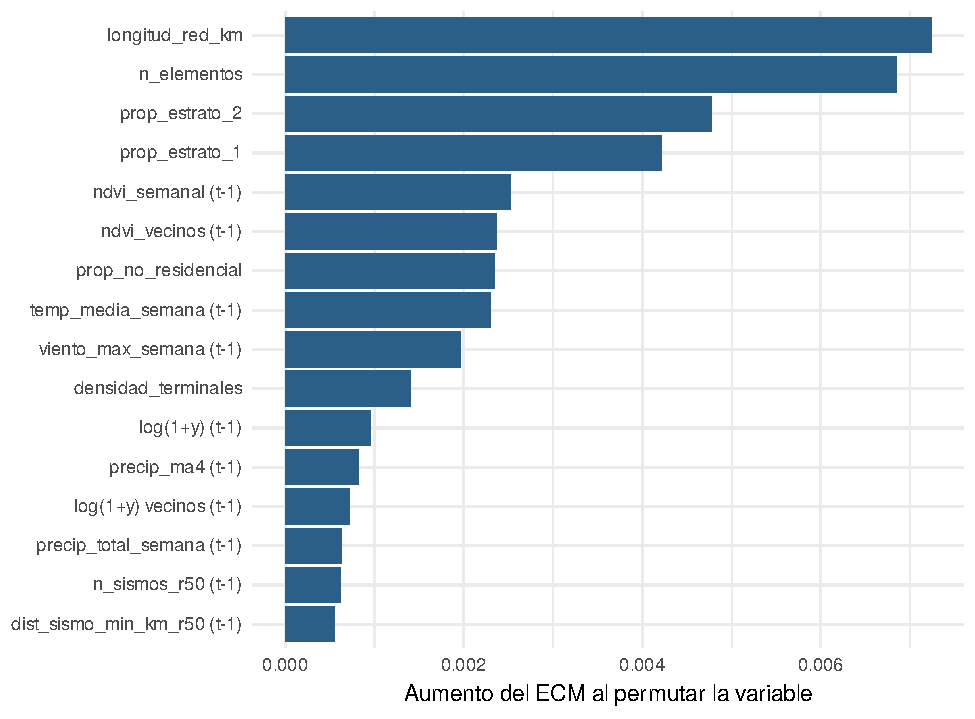
\includegraphics[width=0.85\textwidth]{img/fig_importancia_rf_SAIDI.pdf}
    \caption{Importancia por permutación de las predictoras en el Random Forest ajustado de SAIDI.}
    \label{fig:saidi_rf_imp}
\end{figure}

\begin{figure}[!htbp]
    \centering
    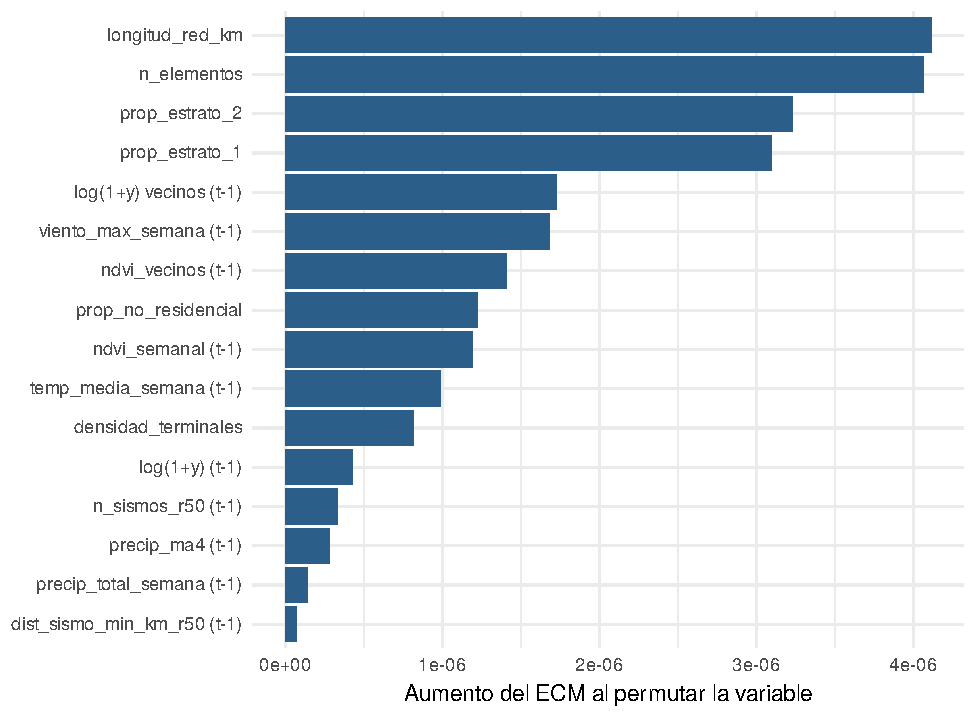
\includegraphics[width=0.85\textwidth]{img/fig_importancia_rf_SAIFI.pdf}
    \caption{Importancia por permutación de las predictoras en el Random Forest ajustado de SAIFI.}
    \label{fig:saifi_rf_imp}
\end{figure}

La convergencia se limita a las variables de \textit{tamaño y forma de la red}: el número de elementos y la longitud de red son las dos primeras en importancia en ambos Random Forest y las más significativas en ambos cortes transversales. Para SAIDI se suma la vegetación (NDVI). Las variables que cambian de semana a semana (clima, NDVI y sismicidad rezagados) no resultan significativas en ningún modelo de panel, lo que es coherente con la escasa ganancia de los modelos sobre la media del cuadrante. Las proporciones de estrato ocupan posiciones altas en el Random Forest pero no son significativas en los modelos lineales; como son atributos fijos de cada cuadrante, es probable que el bosque las use como identificadores del cuadrante, es decir, como sustituto del efecto fijo, más que como un efecto socioeconómico propiamente dicho.

El coeficiente negativo de \texttt{longitud\_red\_km} merece comentario, porque podría leerse como contraintuitivo: una red más extensa expone más activos a falla. Condicionada al número de elementos, la longitud deja de medir exposición y pasa a aproximar el carácter rural y disperso del cuadrante: a igual número de activos, mayor longitud implica menor densidad de usuarios y, por tanto, menor contribución a un indicador ponderado por usuarios afectados. Esta lectura es una hipótesis que los datos no permiten verificar, y el signo no justifica reducir la red como intervención. La antigüedad de los activos, que en la versión anterior del análisis aparecía con signo negativo, ya no se incluye: las fechas de modificación con que se calculaba son en su mayoría de 2026, posteriores al periodo de estudio, y no permiten medir el envejecimiento de la red.

Las Figuras~\ref{fig:saidi_pred_obs} y~\ref{fig:saifi_pred_obs} contrastan los valores observados y pronosticados por FE de cuadrante en el conjunto de prueba. La nube se concentra en una banda estrecha de valores pronosticados para cada cuadrante, mientras los valores observados se dispersan en todo el rango: es la expresión gráfica de que el modelo anticipa el nivel del cuadrante, pero no la magnitud de la semana concreta.

\begin{figure}[!htbp]
    \centering
    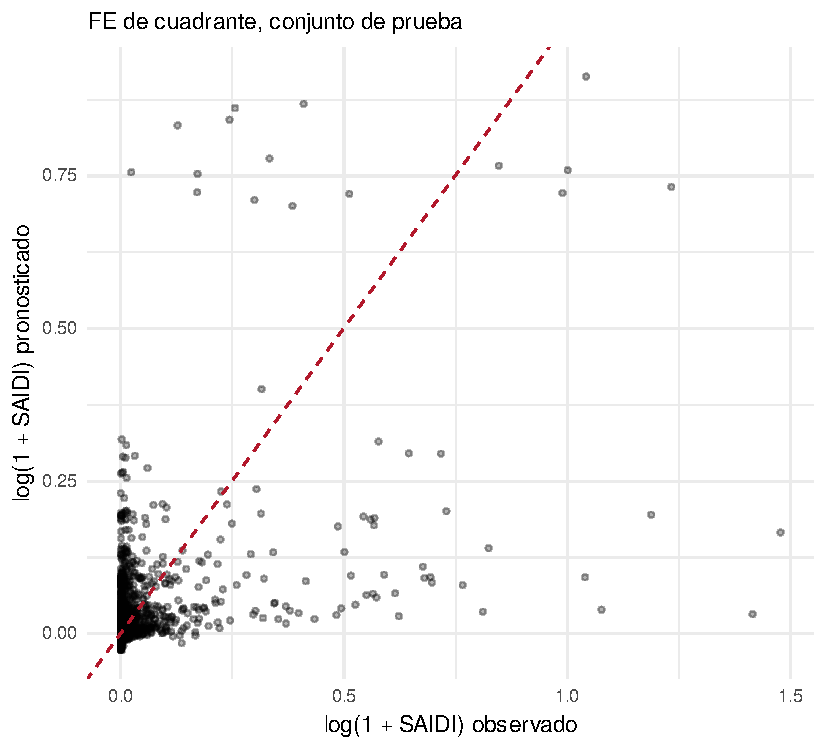
\includegraphics[width=0.62\textwidth]{img/fig_pred_obs_SAIDI.pdf}
    \caption{SAIDI observado frente a pronosticado por FE de cuadrante en el conjunto de prueba (escala $\log(1+y)$).}
    \label{fig:saidi_pred_obs}
\end{figure}

\begin{figure}[!htbp]
    \centering
    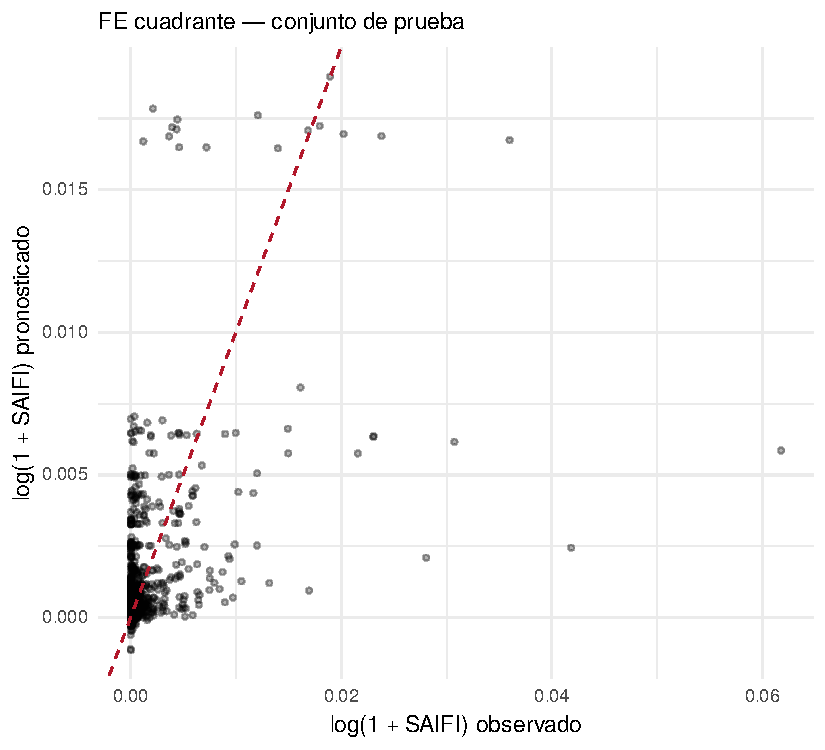
\includegraphics[width=0.62\textwidth]{img/fig_pred_obs_SAIFI.pdf}
    \caption{SAIFI observado frente a pronosticado por FE de cuadrante en el conjunto de prueba (escala $\log(1+y)$).}
    \label{fig:saifi_pred_obs}
\end{figure}

\subsection{Validación fuera de muestra de la priorización territorial}
\label{sec:validacion_ranking}

La Tabla~\ref{tab:captura_ranking} y la Figura~\ref{fig:captura_ranking} presentan la curva de captura definida en la ecuación~\eqref{eq:curva_captura}. El orden construido con la afectación de 2024 se aproxima estrechamente al orden óptimo de 2025. Los diez cuadrantes con mayor afectación en 2024 concentraron el $59{.}6$~\% del SAIDI y el $53{.}2$~\% del SAIFI operativos de 2025, frente a un máximo alcanzable de $61{.}7$~\% y $54{.}6$~\%, respectivamente, y frente al $2{.}9$~\% esperado bajo una selección aleatoria. Con treinta cuadrantes, que representan el $8{.}7$~\% del territorio, el orden histórico capturó el $78{.}5$~\% del SAIDI y el $71{.}7$~\% del SAIFI.

\begin{table}[!htbp]
\centering
\small
\caption{Proporción de la afectación de 2025 capturada por los $k$ primeros cuadrantes, según el criterio de priorización (\%)}
\label{tab:captura_ranking}
\begin{adjustbox}{max width=\linewidth}
\begin{tabular}{l r r r r r}
\toprule
\textbf{Indicador} & \textbf{$k$} & \textbf{Orden 2024} & \textbf{Usuarios del cuadrante} & \textbf{Orden óptimo 2025} & \textbf{Selección aleatoria} \\
\midrule
SAIDI & 10 & 59.6 & 52.2 & 61.7 & 2.9 \\
 & 20 & 67.3 & 59.4 & 74.9 & 5.8 \\
 & 30 & 78.5 & 66.1 & 82.7 & 8.7 \\
 & 47 & 85.4 & 74.4 & 88.9 & 13.7 \\
\addlinespace
SAIFI & 10 & 53.2 & 44.2 & 54.6 & 2.9 \\
 & 20 & 64.9 & 52.6 & 69.0 & 5.8 \\
 & 30 & 71.7 & 57.7 & 76.8 & 8.7 \\
 & 47 & 79.7 & 66.2 & 84.5 & 13.7 \\
\bottomrule
\end{tabular}

\end{adjustbox}

\vspace{2pt}
\noindent\footnotesize\textit{Nota:} $k=47$ corresponde al número de cuadrantes clasificados en prioridad~A y~B. El orden óptimo se construye con los valores observados de 2025 y constituye una cota superior no alcanzable \emph{ex ante}.
\end{table}

\begin{figure}[!htbp]
    \centering
    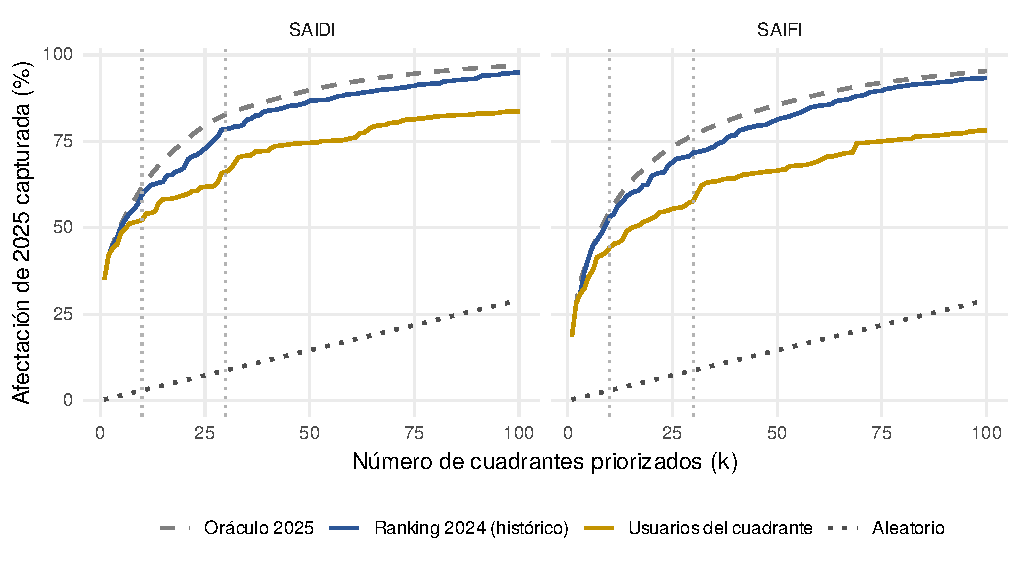
\includegraphics[width=0.95\textwidth]{img/fig_captura_ranking.pdf}
    \caption{Curva de captura de la afectación de 2025 según el criterio de priorización, para los primeros cien cuadrantes. Las líneas verticales punteadas señalan $k=10$ y $k=30$.}
    \label{fig:captura_ranking}
\end{figure}

La historia de interrupciones aportó información que la sola escala del cuadrante no contiene. El orden por número de usuarios capturó entre $7$ y $14$ puntos porcentuales menos que el orden histórico en todos los cortes considerados, lo que indica que la concentración de la afectación no se explica únicamente por el tamaño de la población atendida. La persistencia del orden se refleja también en la correlación de Spearman entre los totales de 2024 y de 2025, de $0{.}93$ para SAIDI y de $0{.}95$ para SAIFI.

El conjunto de cuadrantes prioritarios resultó, además, estable frente a la variación semanal. En el \emph{bootstrap} sobre las semanas de 2024, los cuadrantes 117, 107 y 296 permanecieron entre los diez primeros de SAIDI en más del $98$~\% de las réplicas, y el índice de Jaccard medio entre el conjunto remuestreado y el original fue de $0{.}66$ para SAIDI y de $0{.}78$ para SAIFI. Las sustituciones se concentraron en las últimas posiciones de la lista, lo que sugiere revisar anualmente el límite de la prioridad~A, pero no su núcleo. Dos precisiones delimitan este resultado. La concentración depende de la construcción del indicador: con el SAIDI reconstruido evento a evento, los diez primeros cuadrantes de 2024 capturan el $32{.}4$~\% del SAIDI de 2025, frente a un óptimo del $35{.}7$~\% (Apéndice~\ref{app:robustez_indicador}). Y la captura mide la capacidad del orden para anticipar dónde se concentrará la afectación, no el beneficio de intervenir esos cuadrantes, que requiere una evaluación operativa.

En síntesis, \textbf{para la magnitud de la afectación condicional a la falla, FE de cuadrante es el modelo de menor error en SAIDI y la media histórica del cuadrante en SAIFI}; ambos superan a la persistencia y a Random Forest, pero no se demostró que FE mejore el promedio histórico de cada cuadrante. \textbf{La ocurrencia de falla sí es pronosticable} (AUC de $0{.}84$), aunque esa capacidad proviene de la propensión histórica del cuadrante más que de las variables semanales, y su combinación con la magnitud produce un pronóstico incondicional que mejora al promedio del cuadrante en SAIDI. \textbf{Para la explicación del patrón territorial, SAR es el modelo preferido en SAIDI con todas las matrices de vecindad, y OLS en SAIFI}; el ajuste está dominado por la escala de la red, que actúa sobre la frecuencia y el alcance de los eventos, mientras que la vegetación actúa sobre su duración. Finalmente, \textbf{la priorización territorial construida con un año anticipa la afectación del año siguiente} con una captura cercana a la óptima, cuya magnitud depende de la construcción del indicador.
